\documentclass[../EngineeringJournal_CDavis.tex]{subfiles}

\begin{document}

%%%%%%%%%%%%%%%%%%%%%%%%%%%%%%%%%%%%%%%%%%%%%%%%%%%%%
%%%%%%%%%%%%%%%%%%%%%%%%%%%%%%%%%%%%%%%%%%%%%%%%%%%%%

\chapter[Configuring Basic RIPv2]{Configuring \linebreak[1] Basic RIPv2 \hspace*{\fill}{Jan 31, 2020}}
\noindent\textbf{{Packet Tracer Lab 8} \hspace*{\fill}{\textbf{CIT 167}}}\linebreak[1]
{{Spring 2020} \hspace*{\fill}{Chaz Davis}}                             
%===================================

\hspace{0.2cm}
\begin{tcolorbox}[width=6.3in]
\scriptsize 
- Important Commands for the Lab
  \begin{verbatim}
    enable
    configure terminal

    router rip
    network 192.168.0.0
    version 2
    exit
    exit

    show ip route
    ping 192.168.3.1
    trace 192.168.3.1

    exit
  \end{verbatim}
- Important Concepts
  \begin{itemize}
    \item{Dynamic or adaptive routing} involves automatic updating of the routing
      tables based on information carried by routing protocols.
    \item{Link-state protocols} require that a router inform all the nodes in
      a network of topology changes. Each node shares info regarding
      the nodes it can connect to with the entire network so that each
      node can build its own network map and determine for itself
      the least cost path to any given node.
    \item{RIP} is a distance vector routing protocol which employs the 
      hop count as a routing metric. RIP uses UDP as its transport protocol,
      and is assigned the reserved port number 520.
    \item{auto summarization} a feature which allows RIP to summarize its
      routes to their classful networks automatically.
  \end{itemize}
\end{tcolorbox}
\hspace{0.2cm}
\normalsize  

\newpage

%===================================
\mysection{\textbf{Part 1: Build the Network and Configure Basic Device Settings}}

\begin{wrapfigure}{r}{0.5\textwidth}
\centering
    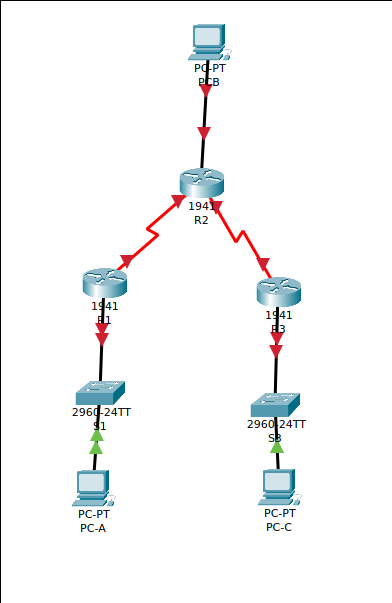
\includegraphics[width=.48\textwidth]{Figures/2020-01-31-112732_392x603_scrot.png}
  \caption{Cabling the Network}
  \label{cable8}
\end{wrapfigure}

\hfill\break
\hfill\break
I did as the Lab specified, I placed three 1941 routers, making sure to turn them off and add on the Serial ports, turning them back on when finished. I then placed two 2960 switches, and then three end user PCs as instructed.
\hfill\break

\noindent\mysubsection{1}{Cable The Network}
I ran the cabling between as shown in the diagram Fig~\ref{cable8}, connecting the correct ports and interfaces.
\hfill\break

\noindent\mysubsection{2}{Initialize the Router and Switch and Configure basic settings for each}
I configured each of the routers and then their serial interfaces, i then configured the switches
\hfill\break

\noindent\mysubsection{3}{Configure PC IP Addressing}
I went to the desktop of each pc and set it up according to the addressing table. See
Fig~\ref{config8}.
\hfill\break

\begin{figure}[!b]\centering
\subfloat[Configuring PC A]{\label{config8PCA}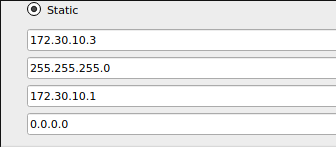
\includegraphics[width=.30\linewidth]{Figures/2020-01-31-120726_336x147_scrot.png}}\par
\subfloat[Configuring PC B]{\label{config8PCB}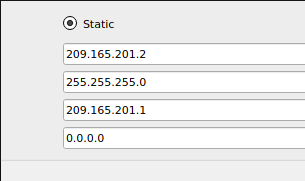
\includegraphics[width=.30\linewidth]{Figures/2020-01-31-120816_305x181_scrot.png}}\hfill 
\subfloat[Configuring PC C]{\label{config8PCC}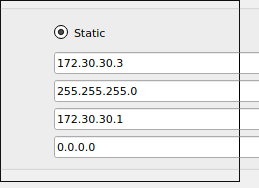
\includegraphics[width=.25\linewidth]{Figures/2020-01-31-120857_259x188_scrot.png}}
\caption{Setting up the PC's according to the addressing Table}
\label{config8}
\end{figure}

\clearpage

\noindent\mysubsection{4}{Test Connectivity}
\\To test connectivity I went to the command prompt on each of the PCs and pinged their
routers. See Fig~\ref{TestConnect8}.

\begin{figure}[!hbt]\centering
\subfloat[]{\label{TestConnect8a}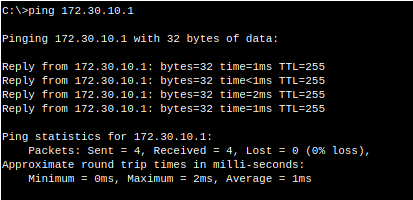
\includegraphics[width=.30\linewidth]{Figures/2020-01-31-122637_413x200_scrot.png}}\hfill 
\subfloat[]{\label{TestConnect8b}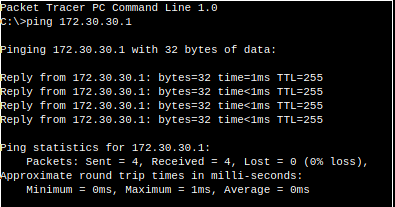
\includegraphics[width=.30\linewidth]{Figures/2020-01-31-122646_395x207_scrot.png}}\par 
\subfloat[]{\label{TestConnect8c}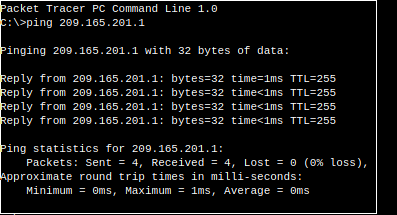
\includegraphics[width=.30\linewidth]{Figures/2020-01-31-122653_397x215_scrot.png}}
\caption{Testing Connectivity}
\label{TestConnect8}
\end{figure}

\newpage

%===================================
\mysection{\textbf{Part 2: Configure and Verify RIPv2 Routing}}


\begin{figure}[!b]\centering
\subfloat[Setting Up RIPv2 on Each
Router]{\label{ipbrief8a}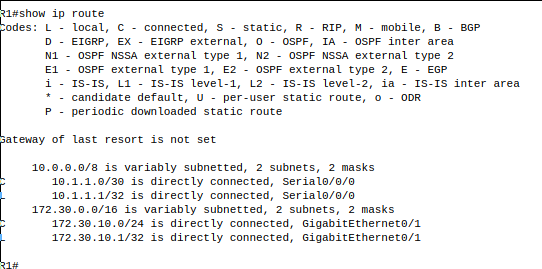
\includegraphics[width=.40\linewidth]{Figures/2020-01-31-123200_542x269_scrot.png}}\hfill
\subfloat[show ip interface brief ran from router
2]{\label{ipbrief8b}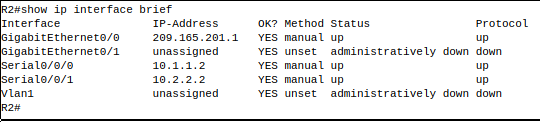
\includegraphics[width=.40\linewidth]{Figures/2020-01-31-123647_540x122_scrot.png}}\par 
\caption{Configuring RIPv2 on the network}
\label{ipbrief8}
\end{figure}

\noindent\mysubsection{1}{Confiugure RIPv2 routing}
I ran the commands for setting up router rip version two on each router see
Fig~\ref{ipbrief8}\subref{ipbrief8a}.
\hfill\break

\noindent\mysubsection{2}{Examine the current state of the network}
\\I ran show ip interface brief from router 2. See Fig~\ref{ipbrief8}\subref{ipbrief8b}.
\hfill\break

\noindent\mysubsection{3}{Disable automatic summarization}
\\I ran No auto-summary from each of the routers, cleared the ip routing tables
\hfill\break

\noindent\mysubsection{4}{Configure and redistribute a default route for internet access}
\\I went to R2 set the default route and then gave the command to distribute the table amongst the network
\hfill\break

\noindent\mysubsection{5}{Verify the routing configuration}
\\I went to R1 and typed show ip route to verify the network configurations as you can
see in Fig~\ref{VerifyRip8}\subref{VerifyRip8a}.
\hfill\break
I then Pinged PC-B from PC-A's interface. See Fig~\ref{VerifyRip8}\subref{VerifyRip8b}.
\hfill\break
Finally, I pinged PC-C from PC-B. Fig~\ref{VerifyRip8}\subref{VerifyRip8c}.

\begin{figure}[!b]\centering
\subfloat[Running show ip route from
R1]{\label{VerifyRip8a}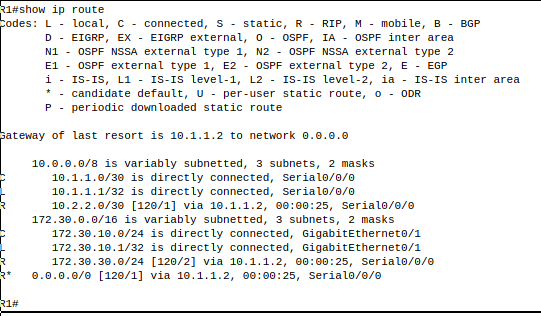
\includegraphics[width=.40\linewidth]{Figures/2020-01-31-124449_541x316_scrot.png}}\par
\subfloat[Pinging PC-B from
PC-A]{\label{VerifyRip8b}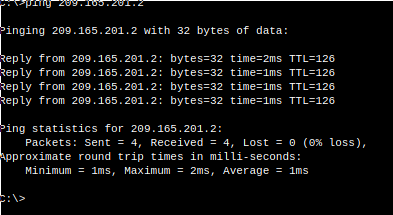
\includegraphics[width=.35\linewidth]{Figures/2020-01-31-124837_393x215_scrot.png}}\hfill 
\subfloat[Pinging PC-C from
PC-A]{\label{VerifyRip8c}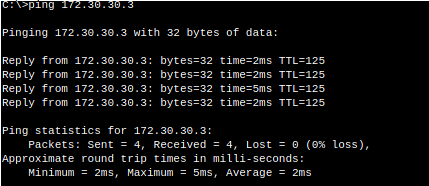
\includegraphics[width=.40\linewidth]{Figures/2020-01-31-125003_429x186_scrot.png}}\par
\caption{Verifying connectivity}
\label{VerifyRip8}
\end{figure}


\newpage
%===================================

\mysection{\textbf{Part 3: Reflection}}

\mysubsection{1}{Why would you turn off auto-summary?}
Route summarization reduces the amount of routing information in the routing tables.  If you are using RIP Version 2, you can turn off automatic summarization by specifying no auto-summary. Disable automatic summarization if you must perform routing between disconnected subnets. When automatic summarization is off, subnets are advertised.

\mysubsection{2}{How did R1 and R3 learn the pathway to the internet?}
they are using rip routing updates from the router default config. RIPv2 multicasts the entire routing table to all adjacent routers at the address 

%===================================

\end{document}

